%%%%%%%%%%%%%%%%%%%%%%%%%%%%%%%%%%%%%%%%%
% Short Sectioned Assignment
% LaTeX Template
% Version 1.0 (5/5/12)
%
% This template has been downloaded from:
% http://www.LaTeXTemplates.com
%
% Original author:
% Frits Wenneker (http://www.howtotex.com)
%
% License:
% CC BY-NC-SA 3.0 (http://creativecommons.org/licenses/by-nc-sa/3.0/)
%
%%%%%%%%%%%%%%%%%%%%%%%%%%%%%%%%%%%%%%%%%

%----------------------------------------------------------------------------------------
%	PACKAGES AND OTHER DOCUMENT CONFIGURATIONS
%----------------------------------------------------------------------------------------

\documentclass[paper=a4, fontsize=11pt]{scrartcl} % A4 paper and 11pt font size

\usepackage[english]{babel} % English language/hyphenation
\usepackage{graphicx,pifont,color} 
\usepackage{amsmath}
\usepackage[byname]{smartref}
%\usepackage{hyperref} %comment out for hardcopy
\usepackage{txfonts}
\usepackage{tocloft}
\usepackage{enumitem}

\usepackage{hyperref}
\usepackage{lhelp}
\usepackage{listings}
\usepackage{float}
\usepackage{xcolor}
\lstset { %
	language=C,
	backgroundcolor=\color{black!5}, % set backgroundcolor
	basicstyle=\footnotesize,% basic font setting
	belowcaptionskip=1\baselineskip,
	breaklines=true,
	frame=L,
	xleftmargin=\parindent,
	showstringspaces=false,
	basicstyle=\footnotesize\ttfamily,
	keywordstyle=\bfseries\color{green!40!black},
	commentstyle=\itshape\color{purple!40!black},
	identifierstyle=\color{blue},
	stringstyle=\color{orange},
	numbers=left,
	stepnumber=1,
}
\usepackage{lipsum} % Used for inserting dummy 'Lorem ipsum' text into the template

\usepackage{sectsty} % Allows customizing section commands
\allsectionsfont{\centering \normalfont\scshape} % Make all sections centered, the default font and small caps

\usepackage{fancyhdr} % Custom headers and footers
\pagestyle{fancyplain} % Makes all pages in the document conform to the custom headers and footers
\fancyhead{} % No page header - if you want one, create it in the same way as the footers below
\fancyfoot[L]{} % Empty left footer
\fancyfoot[C]{} % Empty center footer
\fancyfoot[R]{\thepage} % Page numbering for right footer
\renewcommand{\headrulewidth}{0pt} % Remove header underlines
\renewcommand{\footrulewidth}{0pt} % Remove footer underlines
\setlength{\headheight}{13.6pt} % Customize the height of the header

\numberwithin{equation}{section} % Number equations within sections (i.e. 1.1, 1.2, 2.1, 2.2 instead of 1, 2, 3, 4)
\numberwithin{figure}{section} % Number figures within sections (i.e. 1.1, 1.2, 2.1, 2.2 instead of 1, 2, 3, 4)
\numberwithin{table}{section} % Number tables within sections (i.e. 1.1, 1.2, 2.1, 2.2 instead of 1, 2, 3, 4)

\setlength\parindent{0pt} % Removes all indentation from paragraphs - comment this line for an assignment with lots of text

%----------------------------------------------------------------------------------------
%	TITLE SECTION
%----------------------------------------------------------------------------------------

\newcommand{\horrule}[1]{\rule{\linewidth}{#1}} % Create horizontal rule command with 1 argument of height

\title{	
\normalfont \normalsize 
\textsc{Computer Science Department, UWO} \\ [25pt] % Your university, school and/or department name(s)
\horrule{0.5pt} \\[0.4cm] % Thin top horizontal rule
\huge CS9668\\
Assignment 1 \\ % The assignment title
\horrule{2pt} \\[0.5cm] % Thick bottom horizontal rule
}

\author{Linxiao Wang\\
	250888611} % Your name

\date{\normalsize\today} % Today's date or a custom date

\begin{document}

\maketitle % Print the title

%----------------------------------------------------------------------------------------
%	PROBLEM 1
%----------------------------------------------------------------------------------------

\section*{Problem 1}
Command: host stegosaurus

\begin{figure}[h]
	\centering
	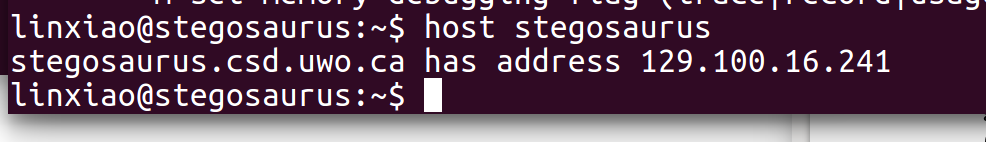
\includegraphics[width=\textwidth]{A1Q1.png}
	\caption{Screen shot of ``host stegosaurus''}
	\label{fig:pingstego}
\end{figure}
\begin{itemize}
\item Symbolic name: stegosaurus.csd.uwo.ca

\item IP address: 129.100.16.241 or
			10000001 01100100 00010000 11110001
			
\item Class: B. Since the IP address in binary starts with "10", it means class B is assigned to the computers in the University's network.

\item Prefix: 129.100 or 10000001 01100100

\item There can be $2^{16} = 65536$ computers in this network.		

\end{itemize}

\section*{Problem 2}
I wrote a program that can generate a list of random IP addresses in the network 129.100. 
\begin{lstlisting}[caption={C code for generating random IP addresses},captionpos=b,label = {lst:generateip}]
#include <stdio.h>
#include <stdlib.h>
#include <time.h>

int main(){
	time_t t;
	srand((unsigned) time(&t));
	FILE* output = fopen("list.txt","w");
	for(int i = 0; i <100; i ++){
		fprintf(output,"129.100.%d.%d\n",rand()%256,rand()%256);
	}
	return 0;
}
\end{lstlisting}

I used the code~\ref{lst:generateip} to generate a list of 100 IP addresses. Then I wrote a script~\ref{lst:pingip} to \textbf{ping} all these IP, and counted how many of them were up.
\begin{lstlisting}[caption={Script for ping all the IP},captionpos=b,label = {lst:pingip}]
#!/bin/bash
# Program name: pingip.sh
date
TEMPFILE=/tmp/tempfile.tmp
echo 0 > $TEMPFILE
cat list.txt |  while read output
do
	ping -c 1 -w 5 "$output">/dev/null
	if [ $? -eq 0 ]; then
		echo "node $output is up"
		counter=$[$(cat $TEMPFILE) + 1]
		echo $counter > $TEMPFILE
	else
		echo "node $output is down"
	fi
done
cat $TEMPFILE
}
\end{lstlisting}

The complete list of IP is long so the following lists the ones that correspond to actual computer.

linxiao@stegosaurus:/data/d1/student/linxiao/CS9868 ./pingip.sh 
Thu Sep 27 14:13:39 EDT 2018
node 129.100.252.82 is up\\
node 129.100.177.10 is up\\
node 129.100.92.225 is up\\
node 129.100.75.165 is up\\
node 129.100.6.219 is up\\
node 129.100.176.110 is up\\
node 129.100.234.251 is up\\
node 129.100.76.255 is up\\
node 129.100.132.28 is up\\
node 129.100.85.22 is up\\
node 129.100.61.221 is up\\
node 129.100.225.23 is up\\

There are 12 out of 100 IPs responded to the ping command. So I assume the ratio of IPs that are used in the network is $12\%$. So my estimation of the size of the network is $65536 \times 12\% \approx 7864$ computers.
%-----------------------------------------------------------------------------

\section*{Problem 3}
Figure~\ref{fig:ipshow} shows the screenshot of the result of command ``ip addr show''. My IP address in the CIDR notation is 129.100.18.146/22.

My IP address in binary is: 10000001 01100100 00010010 10010010/22

Network number:10000001 01100100 000100

Computer number:1010010010

There can be $2^{10} = 1024$ computers in the subnetwork to which my computer is connected.
\begin{figure}[h]
	\centering
	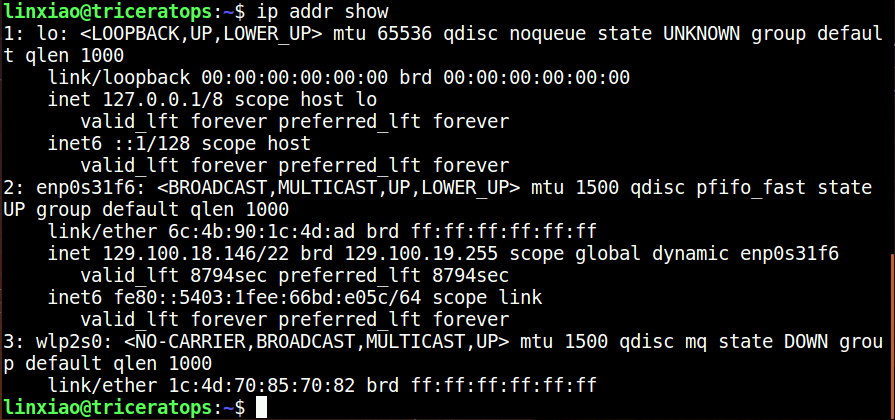
\includegraphics[width=\textwidth]{A1Q3.png}
	\caption{ip addr show}
	\label{fig:ipshow}
\end{figure}

\section*{Problem 4}
Figure~\ref{fig:traceroute} shows the result of maximum number of hops that I can find, the destination is the host of the website ``www.gnu.org'' the IP address of the host is ``208.118.235.148''. Following list shows the possible location of each server that I got from IP2Location.

\begin{figure}[htbp]
	\centering
	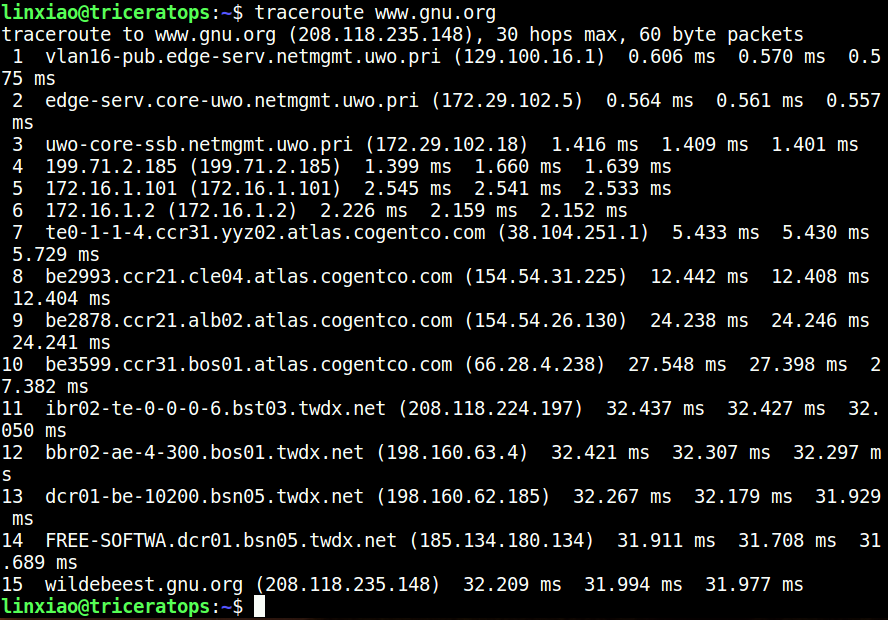
\includegraphics[width=0.7\textwidth]{A1Q4.png}
	\caption{Trace route result}
	\label{fig:traceroute}
\end{figure}
\begin{enumerate}
	\item [1] 129.100.16.1 London,ON,Canada
	\item [2] 172.29.102.5 private IP address
	\item [3] 172.29.102.18 private IP address
	\item [4] 199.71.2.185 London,ON,Canada,N6A 5B7
	\item [5] 172.16.1.101 private IP address
	\item [6] 172.16.1.2 private IP address
	\item [7] 38.104.251.1 Atlanta,Georgia,US,30301
	\item [8] 154.54.31.225 Cleveland,Ohio,US,44101
	\item [9] 154.54.26.130 Albany,New York,US,12201
	\item [10] 66.28.4.238 Miami,Florida,US,33010
	\item [11] 208.118.224.197 Boston,Massachusetts,US,02110
	\item [12] 198.160.63.4 Boston,Massachusetts,US,02210
	\item [13] 198.160.62.185 Boston,Massachusetts,US,02210
	\item [14] 185.134.180.134 Somerville,Massachusetts,US,02143
	\item [15] 208.118.235.148 Boston,Massachusetts,US,02110
\end{enumerate}

\section*{Problem 5}
\subsection*{Part 1}
If A chose a number between 1 to 3, there are two possible choice for B that is different from A. So the possibility of not having the second collision is $\frac{2}{3}$.
\subsection*{Part 2}
For the first $k - 1$ rounds, the possibility of having a collision in each round is always $\frac{1}{3}$, so the possibility of having collision in the all $k - 1$ rounds is $(\frac{1}{3})^{k-1}$. In the $k$-th round, the possibility of not having a collision is $\frac{2}{3}$. So the possibility of exactly k rounds are needed before one of the computers can transmit is
\[(\frac{1}{3})^{k-1} \times \frac{2}{3} = \frac{2}{3^k}\]

\section*{Problem 6}
\section*{Problem 7}
Table~\ref{tab:routingtable} gives the routing table for router $R_1$.
\begin{table}[htbp]
	\centering%	
	\begin{tabular}{|l|l|} \hline 
		Destination & Nest hop  \\ \hline
		132.32.16.10 &deliver direct\\ \hline
		164.80.22.31&deliver direct\\ \hline
		192.10.4.2&192.10.4.16 \\ \hline
		129.1.44.12&129.1.7.12\\ \hline
		194.8.11.55&deliver direct\\ \hline
		196.3.7.4&196.3.7.18\\ \hline	
	\end{tabular}
	\caption{\small Routing table for $R_1$.}
	\label{tab:routingtable}
\end{table}
\section*{Problem 8}
Network 1 packet: 

1. [\textbf{packet header:} MAC address of A, MAC address of $R_1$, control bits of Network 1

\textbf{packet data:} \{\textbf{datagram header:} IP address of A, IP address of B, rest of header. \textbf{datagram data:} 500 bytes\}]

\bigskip
Network 2 packets: 

1. [\textbf{packet header:} MAC address of $R_1$, MAC address of $R_2$, control bits of Network 2

\textbf{packet data:} \{\textbf{datagram header:} IP address of A, IP address of B, rest of header. \textbf{datagram data:} 350 bytes\}]

2. [\textbf{packet header:} MAC address of $R_1$, MAC address of $R_2$, control bits of Network 2

\textbf{packet data:} \{\textbf{datagram header:} IP address of A, IP address of B, rest of header. \textbf{datagram data:} 150 bytes\}]

\bigskip
Network 3 packets: 

1. [\textbf{packet header:} MAC address of $R_2$, MAC address of B, control bits of Network 3

\textbf{packet data:} \{\textbf{datagram header:} IP address of A, IP address of B, rest of header. \textbf{datagram data:} 350 bytes\}]

2. [\textbf{packet header:} MAC address of $R_2$, MAC address of B, control bits of Network 2

\textbf{packet data:} \{\textbf{datagram header:} IP address of A, IP address of B, rest of header. \textbf{datagram data:} 150 bytes\}]


\end{document}